\section{Method}

\subsection{Simple price aware extension of LightGCN}
\begin{figure}
    \centering
    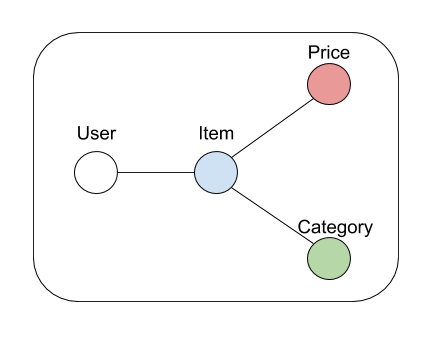
\includegraphics[scale=0.5]{figures/uipc.png}
    \caption{Illustration of the nodes in the simple extension of LightGCN.}   
    \label{fig:uipc}
\end{figure}
We try to extend the implementation of LightGCN by changing the input parameters, where we construct the adjacency matrix containing the users, item, category and price graph, which is illustrated in \autoref{fig:uipc}.
The intuition behind the idea, is that the graph convolutions will capture the values of categories and price, so even if we do not use the embeddings for price and category, they will still influence users and items.
Let the user-item, item-price and item-category interactions matrix be $R \in \mathbb{R}^{I \times U + C + P}$, where $I$ denotes the number of users, $U, C, P$ denotes the number of users, categories and prices.
Each entry of $R_{ui}$ is 1 if $user u$ has rated $item i$. Otherwise it is 0.
If there is a connection in $R_{ic}$ or $R_{ip}$ this value is a hyperparameter $X$ with a value $x>0$, otherwise it is 0. 
The adjacency matrix is obtained as follows:
\begin{gather}
    A = 
    \begin{bmatrix}
        0 & R \\
        R^T & 0
    \end{bmatrix}
\end{gather}
The embeddings for users and price are calculated as follows,
\begin{equation}
    E^{(k+1)} = (D^{\frac{1}{2}}AD^{\frac{1}{2}}E^{(k)}),
\end{equation}
where $A$ is the adjacency matrix containing users, items, categories and price, and $D$ is a $(I + U + C + P)$ diagonal matrix, where $D_{ii}$ denotes the sum of the $i-th$ row in the adjacency matrix $A$. 
The $0th$ layer embedding $E^{(0)} \in R^{(I + U + C + P)\times T}$, where $T$ is the embedding size.
We do not change anything else in LightGCN in this method.